%%%%%%%%%%%%%%%%%%%%%%%%%%%%%%%%%%%%%%%%%
% Short Sectioned Assignment
% LaTeX Template
% Version 1.0 (5/5/12)
%
% This template has been downloaded from:
% http://www.LaTeXTemplates.com
%
% Original author:
% Frits Wenneker (http://www.howtotex.com)
%
% License:
% CC BY-NC-SA 3.0 (http://creativecommons.org/licenses/by-nc-sa/3.0/)
%
%%%%%%%%%%%%%%%%%%%%%%%%%%%%%%%%%%%%%%%%%

%----------------------------------------------------------------------------------------
%	PACKAGES AND OTHER DOCUMENT CONFIGURATIONS
%----------------------------------------------------------------------------------------

\documentclass[paper=a4, fontsize=11pt]{scrartcl} % A4 paper and 11pt font size
\usepackage[margin=0.7in]{geometry}
\usepackage[T1]{fontenc} % Use 8-bit encoding that has 256 glyphs
\usepackage{fourier} % Use the Adobe Utopia font for the document - comment this line to return to the LaTeX default
\usepackage[english]{babel} % English language/hyphenation
\usepackage{amsmath,amsfonts,amsthm} % Math packages

\usepackage{lipsum} % Used for inserting dummy 'Lorem ipsum' text into the template

\usepackage{sectsty} % Allows customizing section commands
\allsectionsfont{\bfseries\sffamily\scshape} % Make all sections centered, the default font and small caps

\usepackage{fancyhdr} % Custom headers and footers
\pagestyle{fancyplain} % Makes all pages in the document conform to the custom headers and footers
\fancyhead{} % No page header - if you want one, create it in the same way as the footers below
\fancyfoot[L]{} % Empty left footer
\fancyfoot[C]{} % Empty center footer
\fancyfoot[R]{\thepage} % Page numbering for right footer
\renewcommand{\headrulewidth}{0pt} % Remove header underlines
\renewcommand{\footrulewidth}{0pt} % Remove footer underlines
\setlength{\headheight}{13.6pt} % Customize the height of the header

\numberwithin{equation}{section} % Number equations within sections (i.e. 1.1, 1.2, 2.1, 2.2 instead of 1, 2, 3, 4)
\numberwithin{figure}{section} % Number figures within sections (i.e. 1.1, 1.2, 2.1, 2.2 instead of 1, 2, 3, 4)
\numberwithin{table}{section} % Number tables within sections (i.e. 1.1, 1.2, 2.1, 2.2 instead of 1, 2, 3, 4)

\setlength\parindent{0pt} % Removes all indentation from paragraphs - comment this line for an assignment with lots of text

\usepackage[english]{babel}
\usepackage{graphicx}
\usepackage{listings}
\usepackage{amsmath}
\usepackage{listings}
\usepackage{color}
\usepackage{caption}
\usepackage{subcaption}

\definecolor{dkgreen}{rgb}{0,0.6,0}
\definecolor{gray}{rgb}{0.5,0.5,0.5}
\definecolor{mauve}{rgb}{0.58,0,0.82}

\lstset{frame=tb,
  language=Java,
  aboveskip=3mm,
  belowskip=3mm,
  showstringspaces=false,
  columns=flexible,
  basicstyle={\small\ttfamily},
  numbers=none,
  numberstyle=\tiny\color{gray},
  keywordstyle=\color{blue},
  commentstyle=\color{dkgreen},
  stringstyle=\color{mauve},
  breaklines=true,
  breakatwhitespace=true,
  tabsize=3
}

%----------------------------------------------------------------------------------------
%	TITLE SECTION
%----------------------------------------------------------------------------------------

\newcommand{\horrule}[1]{\rule{\linewidth}{#1}} % Create horizontal rule command with 1 argument of height

\title{	
\normalfont \normalsize 
\textsc{University of Southern California, Computer Science} \\ [25pt] % Your university, school and/or department name(s)
\horrule{0.5pt} \\[0.4cm] % Thin top horizontal rule
\huge Machine Learning: HomeWork 5 \\ % The assignment title
\horrule{2pt} \\[0.5cm] % Thick bottom horizontal rule
}

\author{Rohit Kondekar\\
740-581-9473} % Your name

\date{\normalsize\today} % Today's date or a custom date
\allowdisplaybreaks
\begin{document}

\maketitle % Print the title


%----------------------------------------------------------------------------------------
%	PROBLEM 1
%----------------------------------------------------------------------------------------
\section{Question: Principal Component Analysis }
\subsection{Deriving PCA in terms of minimum reconstruction error}
\subsubsection{}
This can be solved by working on single principal direction and then generalizing it. Let $U_{j}\epsilon R^{D}$ to denote the basis vector in jth principal direction. Let  $x_{i}\epsilon R^{D}$ high dimension feature vector and $z_{i}\epsilon R^{d}$ low dimension feature vector. Let $\hat{z}_{j}\epsilon R^{N}$ to denote jth component of all low dimensional feature vector.

\begin{align*} 
J(U_{1},z_{1}) &=  \sum_{i=1}^{N}||x_{i}-z_{i1}U_{i}||^{2}\\
&= \sum_{i=1}^{N} (x_{i}-z_{i1}U_{i})^{T}(x_{i}-z_{i1}U_{i})\\
&= \sum_{i=1}^{N} (x_{i}^{T}x_{i} - 2z_{i1}U_{i}^{T}x_{i} + z_{i1}^{2}) ~~~~~~\textsl{$z_{i1}$ is a scalar}\\
\dfrac{\partial J(U_{1},z_{1})}{\partial z_{i1}} &= -2U_{1}^{T}x_{i} + 2z_{i1} = 0\\
z_{i1} &= U_{1}^{T}x_{i}
\end{align*}

\subsubsection{}
Substituting value obtained in earlier eqution in the cost function.
\begin{align*} 
J &= \sum_{i=1}^{N} ( x_{i}^{T}x_{i} - 2z_{i1}U_{i}^{T}x_{i} + z_{i1}^{2} )\\
&= \sum_{i=1}^{N} ( x_{i}^{T}x_{i} - 2z_{i1}^{2} + z_{i1}^{2} )\\
&= \sum_{i=1}^{N} ( x_{i}^{T}x_{i} - z_{i1}^{2} )\\
\end{align*}

Minimizing J is same as maximizing $z_{i1}^{2}$
\begin{align*} 
\sum_{i=1}^{N} z_{i1}^{2} &= \sum_{i=1}^{N} U_{1}x_{i}x_{i}^{T}U_{i}\\
&= U_{1}^{T}\Sigma U_{i}
\end{align*}

So the optimization equation is:
\begin{align*} 
\textsc{Max}  ~~~~U_{1}\Sigma U_{i}\\
\textsf{Constraint}~~~~~ U^{T}_{1}U_{1}=1\\
\end{align*}

Lagrange Multiplier:
\begin{align*} 
L &= U_{1}\Sigma U_{i} + \lambda (U^{T}_{1}U_{1}-1)\\
\dfrac{\partial L}{\partial U_{1}} &= 2\Sigma U_{1} - 2\lambda_{1}U_{1}=0\\
\Sigma U_{1} &= \lambda_{1}U_{1}
\end{align*}

This proves that $U_{1}$ is an eigen vector and U is matrix of eigen vectors of $\Sigma$

\subsection{Projecting a Gaussian distribution}
\subsubsection{}

$x \sim N(0,\Sigma)$ : x is a Gaussian Random Vector (Multivariate Gaussian) of D jointly Gaussian RVs.\\

$z = p^{T}x$ : is a linear combination of D random variables. Which comes out to be Univariate Gaussian.

As z, is normally distributed with mean 0, the value of variance would be equal to the second order moment.

\begin{align*} 
\sigma_{z}^{2} = E[z^{2}] &= E[p^{T}XX^{T}p]\\
&= p^{T}\Sigma p
\end{align*}

Therefore, z is Normally distributed with $N(0,p^{T}\Sigma p)$\\

Entropy of z is given by :\\

\begin{align*} 
H(z) &= -\int_{-\infty}^{-\infty}f(z)\log(\dfrac{e^{\dfrac{-z^{2}}{2\sigma^{2}}}}{\sqrt{2\Pi \sigma^{2}}}) ~~~~ \textsl{where $\sigma^{2}$ is given by $p^{T}\Sigma p$}\\
&= \int_{-\infty}^{-\infty}f(z)\log(\sqrt{2\Pi \sigma^{2}})dz + \int_{-\infty}^{-\infty}f(z)\dfrac{z^{2}}{2\sigma^{2}}\log_{2}(e) dz\\
H(z) &= \dfrac{1}{2}\log(2\Pi \sigma^{2}) + \dfrac{1}{2}\log_{2}(e)
\end{align*}

So we need to maximize entropy given the constrain that $p^{T}p=1$. Therefore optimization equation with langrange multipler:
\begin{align*} 
L &= \dfrac{1}{2}\log(2\Pi p^{T}\Sigma p) + \dfrac{1}{2}\log_{2}(e) + \lambda (p^{T}p-1)\\
\dfrac{\partial L}{\partial p} &= \dfrac{\Sigma p}{p^{T}\Sigma p} + 2\lambda p = 0\\
\Sigma p &= (\lambda^{'}p^{T}\Sigma p)p  ~~~~ \textsl{As $p^{T}\Sigma p$ is scalar}\\
\Sigma p &= \lambda^{''}p
\end{align*}

So here we can see that to maximize Entropy of z, $p^{*}$ should be eigen vectors of $\Sigma$.

\subsubsection{}
As from the equation in the first part:

\begin{align*} 
H(z) &= \dfrac{1}{2}\log(2\Pi \sigma^{2}) + \dfrac{1}{2}\log_{2}(e)
\end{align*}

Maximizing Entropy is same is maximizing Variance $\sigma^{2}_{z}$ which we have obtained in the first part. So by maximizing variance we are maximing the entropy. Therefore $p^{*}$ maximizes variance of z.




%----------------------------------------------------------------------------------------
%	PROBLEM 2
%----------------------------------------------------------------------------------------
\section{Hidden Markov Models}

Transition Probabilities:\\\\
\begin{tabular}{l*{3}{c}}
\textbf{} & \textbf{S1} &  \textbf{S2}  \\
\hline
\textbf{S1} & 0.7 & 0.3\\
\textbf{S2} & 0.3 & 0.7
\end{tabular}\\\\


Emission Probabilities:\\\\
\begin{tabular}{l*{5}{c}}
\textbf{} & \textbf{A} &  \textbf{C} & \textbf{G} & \textbf{T} \\
\hline
\textbf{S1} & 0.4 & 0.1 & 0.4 & 0.1\\
\textbf{S2} & 0.1 & 0.4 & 0.1 & 0.4
\end{tabular}\\\\

Initial State Distribution $\pi$:\\\\
$\pi_{1} = 0.5$\\
$\pi_{2} = 0.5$\\

Given Sequence: e = CGTCAG

\subsection{}
Forward Probabilities:\\\\
C:\\
$\alpha_{1}(S_{1}) = 0.5*0.1 = 0.05$\\
$\alpha_{1}(S_{2}) = 0.5*0.4 = 0.20$\\

G:\\
$\alpha_{2}(S_{1}) = (0.05*0.7*0.4)+ (0.20*0.3*0.4)= 0.038$\\
$\alpha_{2}(S_{2}) = (0.05*0.3*0.1)+ (0.20*0.7*0.1)= 0.0155$\\

T:\\
$\alpha_{3}(S_{1}) = (0.038*0.7*0.1)+ (0.0155*0.3*0.1)= 0.003125$\\
$\alpha_{3}(S_{2}) = (0.038*0.3*0.4)+ (0.0155*0.7*0.4)= 0.0089$\\

C:\\
$\alpha_{4}(S_{1}) = (0.003125*0.7*0.1)+ (0.0089*0.3*0.1)= 0.00048575$\\
$\alpha_{4}(S_{2}) = (0.003125*0.3*0.4)+ (0.0089*0.7*0.4)= 0.002867$\\

A:\\
$\alpha_{5}(S_{1}) = (0.00048575*0.7*0.4)+ (0.002867*0.3*0.4)= 0.00048005$\\
$\alpha_{5}(S_{2}) = (0.00048575*0.3*0.1)+ (0.002867*0.7*0.1)= 0.0002152625$\\

G:\\
$\alpha_{6}(S_{1}) = (0.00048005*0.7*0.4)+ (0.0002152625*0.3*0.4)= 0.0001602455$\\
$\alpha_{6}(S_{2}) = (0.00048005*0.3*0.1)+ (0.0002152625*0.7*0.1)= 0.000029469875$\\

Alphas:\\\\
\begin{tabular}{l*{7}{c}}
\textbf{T} & \textbf{1} &  \textbf{2} & \textbf{3} & \textbf{4} & \textbf{5} & \textbf{6} \\
\hline
\textbf{$\alpha_{t}(S1)$} & 0.05 & 0.038 & 0.003125 & 0.00048575 & 0.00048005 & 0.0001602455\\
\textbf{$\alpha_{t}(S2)$} & 0.20 & 0.0155 & 0.0089 & 0.002867 & 0.0002152625 & 0.000029469875
\end{tabular}\\\\

Therefore, $P(e|\theta)=0.0001602455+0.000029469875 = 0.000189715375$

\subsection{}
Backward Probabilities:\\\\


$\beta_{6}(S_{1}) = 1$\\
$\beta_{6}(S_{2}) = 1$\\

G:\\
$\beta_{5}(S_{1}) = (1*0.4*0.7) + (1*0.1*0.3) = 0.31$\\
$\beta_{5}(S_{2}) = (1*0.4*0.3) + (1*0.1*0.7) = 0.19$\\


A:\\
$\beta_{4}(S_{1}) = (0.31*0.4*0.7) + (0.19*0.1*0.3) = 0.0925$\\
$\beta_{4}(S_{2}) = (0.31*0.4*0.3) + (0.19*0.1*0.7) = 0.0505$\\

C:\\
$\beta_{3}(S_{1}) = (0.0925*0.1*0.7) + (0.0505*0.4*0.3) = 0.012535$\\
$\beta_{3}(S_{2}) = (0.0925*0.1*0.3) + (0.0505*0.4*0.7) = 0.016915$\\

T:\\
$\beta_{2}(S_{1}) = (0.012535*0.1*0.7) + (0.016915*0.4*0.3) = 0.00290725$\\
$\beta_{2}(S_{2}) = (0.012535*0.1*0.3) + (0.016915*0.4*0.7) = 0.00511225$\\


G:\\
$\beta_{1}(S_{1}) = (0.00290725*0.4*0.7) + (0.00511225*0.1*0.3) = 0.0009673975$\\
$\beta_{1}(S_{2}) = (0.00290725*0.4*0.3) + (0.00511225*0.1*0.7) = 0.0007067275$\\




Beta:\\\\
\begin{tabular}{l*{7}{c}}
\textbf{T} & \textbf{1} &  \textbf{2} & \textbf{3} & \textbf{4} & \textbf{5} & \textbf{6} \\
\hline
\textbf{$\beta_{t}(S1)$} & 0.0009673975 & 0.00290725 & 0.012535 & 0.0925 & 0.31 & 1\\
\textbf{$\beta_{t}(S2)$} & 0.0007067275 & 0.00511225 & 0.016915 & 0.0505 & 0.19 & 1
\end{tabular}\\\\

Alphas:\\\\
\begin{tabular}{l*{7}{c}}
\textbf{T} & \textbf{1} &  \textbf{2} & \textbf{3} & \textbf{4} & \textbf{5} & \textbf{6} \\
\hline
\textbf{$\alpha_{t}(S1)$} & 0.05 & 0.038 & 0.003125 & 0.00048575 & 0.00048005 & 0.0001602455\\
\textbf{$\alpha_{t}(S2)$} & 0.20 & 0.0155 & 0.0089 & 0.002867 & 0.0002152625 & 0.000029469875
\end{tabular}\\\\


Gamma: $\gamma_{t}(j) = \dfrac{\alpha_{t}(j)\beta_{t}(j)}{\sum_{j}\alpha_{t}(j)\beta_{t}(j)}$

Let Gamma' = $\gamma_{t}^{'}(j) = \alpha_{t}(j)\beta_{t}(j)$\\

\begin{tabular}{l*{7}{c}}
\textbf{T} & \textbf{1} &  \textbf{2} & \textbf{3} & \textbf{4} & \textbf{5} & \textbf{6} \\
\hline
\textbf{$\gamma_{t}^{'}(S1)$} & 0.000048369875 & 0.000110475500 & 0.000039171875 & 0.000044931875 & 0.000148815500 & 0.000160245500\\
\textbf{$\gamma_{t}^{'}(S2)$} & 0.000141345500 & 0.000079239875 & 0.000150543500 & 0.000144783500 & 0.000040899875 & 0.000029469875
\end{tabular}\\\\


\begin{tabular}{l*{7}{c}}
\textbf{T} & \textbf{1} &  \textbf{2} & \textbf{3} & \textbf{4} & \textbf{5} & \textbf{6} \\
\hline
\textbf{$P_{t}(S1)$} & 0.254960227 & 0.582322334 & 0.206477071 & 0.236838343 & 0.784414547 & 0.844662695\\
\textbf{$P_{t}(S2)$} & 0.745039773 & 0.417677666 & 0.793522929 & 0.763161657 & 0.215585453 & 0.155337305
\end{tabular}\\\\

\subsection{}

Veterbi Algorithm:\\

$\delta$ Matrix:\\\\
\begin{tabular}{l*{7}{c}}
\textbf{T} & \textbf{1} &  \textbf{2} & \textbf{3} & \textbf{4} & \textbf{5} & \textbf{6} \\
\hline
\textbf{$\delta_{t}(S1)$} & 0.05 & 0.024 & 0.00168 & 1.176E-4 & 1.3171E-4 & 3.6879359E-5 \\
\textbf{$\delta_{t}(S2)$} & 0.2 & 0.01399 & 0.003919 & 0.001097599 & 7.68319E-5 & 5.378239E-6
\end{tabular}\\\\


$\Psi$ Matrix:\\\\
\begin{tabular}{l*{7}{c}}
\textbf{T} & \textbf{1} &  \textbf{2} & \textbf{3} & \textbf{4} & \textbf{5} & \textbf{6} \\
\hline
\textbf{$\Psi_{t}(S1)$} & 0.0 & 2.0 & 1.0 & 1.0 & 2.0 & 1.0 \\
\textbf{$\Psi_{t}(S2)$} & 0.0 & 2.0 & 2.0 & 2.0 & 2.0 & 2.0
\end{tabular}\\\\

Sequence Obtained by Veterbi Algorithm:\\
2,2,2,2,2,1\\

Sequence of most likely states estimated independently:\\
2,1,2,2,1,1\\

So they are not same, so it doesn't happen in this example.\\

\begin{lstlisting}
//Viterbi.java
double[][] a = {{0,0,0},{0,0.7,0.3},{0,0.3,0.7}};
		double[][] b = {{0,0,0,0,0},{0,0.4,0.1,0.4,0.1},{0,0.1,0.4,0.1,0.4}};
		
		double[] pi = {0,0.5,0.5};
		
		double[][] delta = new double[3][7];
		double[][] si = new double[3][7];
		
		delta[1][1] = pi[1]*b[1][2];
		delta[2][1] = pi[2]*b[2][2];
		si[1][1] = 0;
		si[2][1] = 0;
		
		int[] val = {0,2,3,4,2,1,3};
		
		for(int t=2;t<=6;t++){
			
			for(int j=1;j<=2;j++){
				
				double val1 = delta[1][t-1]*a[1][j]*b[j][val[t]];
				double val2 = delta[2][t-1]*a[2][j]*b[j][val[t]];
				
				if(val1>val2){
					delta[j][t] = val1;
					si[j][t] = 1;
				}
				else{
					delta[j][t] = val2;
					si[j][t] = 2;
				}
			}
			
		}
		
		for (int i = 1; i < delta.length; i++) {
			for (int j = 1; j < delta[1].length; j++) {
				System.out.print(delta[i][j]+" , ");
			}
			System.out.println();
		}
		
		
		for (int i = 1; i < si.length; i++) {
			for (int j = 1; j < si[1].length; j++) {
				System.out.print(si[i][j]+" , ");
			}
			System.out.println();
		}
	}
\end{lstlisting}


\subsection{}

Alphas:\\\\
\begin{tabular}{l*{7}{c}}
\textbf{T} & \textbf{1} &  \textbf{2} & \textbf{3} & \textbf{4} & \textbf{5} & \textbf{6} \\
\hline
\textbf{$\alpha_{t}(S1)$} & 0.05 & 0.038 & 0.003125 & 0.00048575 & 0.00048005 & 0.0001602455 \\
\textbf{$\alpha_{t}(S2)$} & 0.20 & 0.0155 & 0.0089 & 0.002867 & 0.0002152625 & 0.000029469875
\end{tabular}\\\\


Forward Probabilities for all possible emissions:\\

For A:\\
$\alpha_{T+1}(S1) = (0.0001602455*0.7*0.4)+(0.000029469875*0.3*0.4) = 0.00004840512$\\
$\alpha_{T+1}(S2) = (0.0001602455*0.3*0.1)+(0.000029469875*0.7*0.1) = 0.00000687025$\\\\

For C:\\
$\alpha_{T+1}(S1) = (0.0001602455*0.7*0.1)+(0.000029469875*0.3*0.1) = 0.00001210128$\\
$\alpha_{T+1}(S2) = (0.0001602455*0.3*0.4)+(0.000029469875*0.7*0.4) = 0.00002748102$\\

For G:\\
$\alpha_{T+1}(S1) = (0.0001602455*0.7*0.4)+(0.000029469875*0.3*0.4) = 0.00004840512$\\
$\alpha_{T+1}(S2) = (0.0001602455*0.3*0.1)+(0.000029469875*0.7*0.1) = 0.00000687025$\\\\

For T:\\
$\alpha_{T+1}(S1) = (0.0001602455*0.7*0.1)+(0.000029469875*0.3*0.1) = 0.00001210128$\\
$\alpha_{T+1}(S2) = (0.0001602455*0.3*0.4)+(0.000029469875*0.7*0.4) = 0.00002748102$\\

P(A) = P(G) = 0.00005527537\\
P(C) = P(T) = 0.0000395823 \\\\

Hence A or G are mostly likely to be the next symbol. (Equally Likely).
%----------------------------------------------------------------------------------------
%	PROBLEM 3
%----------------------------------------------------------------------------------------
\section{Sample questions}
\subsection{Expection Maximization}

Deriving Generic EM Model to work on:
\begin{align*} 
\sum_{i=1}^{N} \log p(x_{i}|\theta) &= \sum_{i=1}^{N} \log \sum_{k=1}^{K} p(x_{i},z_{k}|\theta)\\
\end{align*}
Let $Q_{i}$ be distribution over z's s.t. $\sum_{k=1}^{K} Q_{i}(z_{k}) = 1$ and $Q_{i}>=0$. Therefore:


\begin{align*} 
&= \sum_{i=1}^{N} \log \sum_{k=1}^{K} Q_{i}(z_{k}) \dfrac{p(x_{i},z_{k}|\theta)}{Q_{i}(z_{k})} \\
&\geq \sum_{i=1}^{N} \sum_{k=1}^{K} Q_{i}(z_{k}) \log \dfrac{p(x_{i},z_{k}|\theta)}{Q_{i}(z_{k})} ~~~~~\textsl{Using Jenson's Inequality}
\end{align*}

For this to be a tight bound, $E[x]=x$ should be satisfied, i.e. x is constant. Therefore:\\
E Step:

\begin{align*} 
\dfrac{p(x_{i},z_{k}|\theta)}{Q_{i}(z_{k})} &= c\\
Q_{i}(z_{k}) &=  \dfrac{p(x_{i},z_{k}|\theta)}{c}\\
Q_{i}(z_{k}) &= \dfrac{p(x_{i},z_{k}|\theta)}{\sum_{k=1}^{K} p(x_{i},z_{k}|\theta) } ~~~~~~~~~ As \sum_{k=1}^{K} Q_{i}(z_{k}) = 1\\
&= \dfrac{p(x_{i},z_{k}|\theta)}{p(x_{i}|\theta) }\\
Q_{i}(z_{k}) &= p(z_{k}|x_{i},\theta)\\
&= \dfrac{p(x_{i}|z_{k},\theta)p(z_{k}|\theta)}{\sum_{k=1}^{K} p(x_{i}|z_{k},\theta) } ~~~~~~~ \textsl{Bayes Rule}\\
\end{align*}

M Step:
\begin{align*} 
\theta &= \textsf{argmax}_{\theta} \sum_{i=1}^{N} \sum_{k=1}^{K} Q_{i}(z_{k}) \log \dfrac{p(x_{i},z_{k}|\theta)}{Q_{i}(z_{k})}
\end{align*}


Gaussian Mixture Models:\\\\
E Step: $Q_{i}(z_{k})$ is given by $p(z_{k}|x_{i},\theta)$, the responsibility that cluster k takes data point i.

\begin{align*} 
Q_{i}(z_{k}) &= \dfrac{p(x_{i}|z_{k},\theta)p(z_{k}|\theta)}{\sum_{k=1}^{K} p(x_{i}|z_{k},\theta) }\\
Q_{i}(z_{k}) = r_{ik} &= \dfrac{w_{k}N(x_{i}|\mu_{k},\Sigma_{k}^{2})}{\sum_{k'=1}^{K} w_{k'}N(x_{i}|\mu_{k'},\Sigma_{k'}^{2})}
\end{align*}

M Step:
\begin{align*} 
\sum_{i=1}^{N} \sum_{k=1}^{K} Q_{i}(z_{k}) \log \dfrac{p(x_{i},z_{k}|\theta)}{Q_{i}(z_{k})} &= \sum_{i=1}^{N} \sum_{k=1}^{K} r_{ik} \log \dfrac{\dfrac{1}{(2\pi)^{n/2}|\Sigma_{k}^{-1}|^{1/2})}exp(\dfrac{-1}{2}((x_{i}-\mu_{k})^{T}\Sigma_{k}^{-1} (x_{i}-\mu_{k})))w_{k}}{r_{ik}}
\end{align*}

Solving for $\mu_{k}$

\begin{align*} 
\bigtriangledown_{ \mu_{k}} (\sum_{i=1}^{N} -r_{ik}\dfrac{1}{2}(x_{i}-\mu_{k})^{T}\Sigma_{k}^{-1} (x_{i}-\mu_{k}))\\
\mu_{k} &= \dfrac{\sum_{i=1}^{N}r_{ik}x_{i}}{r_{k}}
\end{align*}

Solving for $\Sigma_{k}$
\begin{align*} 
\bigtriangledown_{\Sigma_{k}} (\sum_{i=1}^{N} -r_{ik}\dfrac{1}{2}(x_{i}-\mu_{k})^{T}\Sigma_{k}^{-1} (x_{i}-\mu_{k}))\\
\Sigma_{k} &= \dfrac{\sum_{i=1}^{N}r_{ik}(x_{i}-\mu_{k})(x_{i}-\mu_{k})^{T}}{r_{k}}
\end{align*}


Solving for $w_{k}$
\begin{align*} \\
w_{k} &= \dfrac{1}{N}\sum_{i=1}^{N}r_{ik}
\end{align*}


\section{Dimensionality Reduction}
\subsection{}
In Cordinate Component Analysis, all the principal components are just the dimensions of the data. Whereas in PCA, the principal components are the eigen vectors of the covariance matrix. This can have a serious impact because, CCA may not find much covariance in direction of just the dimensions and may lead to no reduction in dimensionality, whereas in PCA it finds the component with the highest variance with restriction of they being orthogonal.

\subsection{}
CCA and PCA may lead to same solution when the data is distributed just around certain dimension of data itself, thereby giving the principal component the dimension of data itself, in case of PCA.

E.g. 2 dimensional data:


\begin{figure}[!htbp]
\centering
\begin{subfigure}{.5\textwidth}
  \centering
  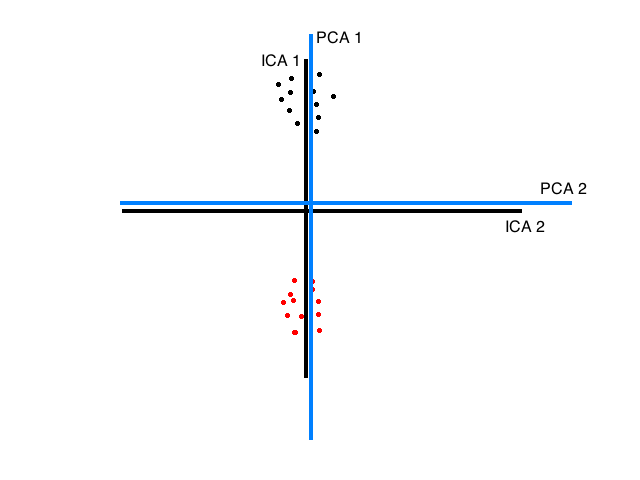
\includegraphics[width=.6\linewidth]{../figures/ica-pca1.png}
  \label{fig:sub1}
\end{subfigure}%
\begin{subfigure}{.5\textwidth}
  \centering
  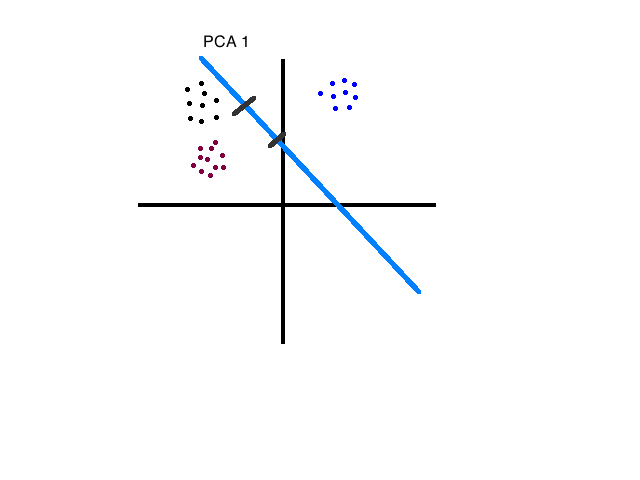
\includegraphics[width=.8\linewidth]{../figures/ica-pca2.png}
  \label{fig:sub2}
\end{subfigure}
\caption{ICA and PCA comparison, second figure shows the disadvantage}
\label{fig:test}
\end{figure}





\newpage
\section{Programming (PCA)}
\subsection{}
\subsection{}

\subsection{}
\begin{figure}[h!]
  \centering
    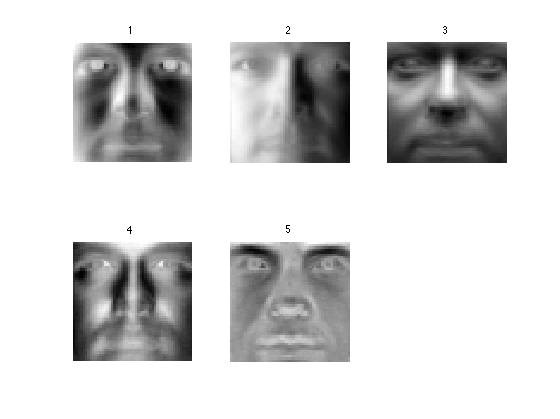
\includegraphics[width=0.75\textwidth]{../figures/eigenFaces.png}
  \caption{Eigen Faces}
\end{figure}


\subsection{}
\subsubsection{Linear SVM}
Validation Linear SVM : Test Subset =1 d =20 C =4 Avg Validation Accuracy =83.1532\\
Validation Linear SVM : Test Subset =2 d =20 C =4 Avg Validation Accuracy =82.2948\\
Validation Linear SVM : Test Subset =3 d =20 C =4 Avg Validation Accuracy =82.2948\\
Validation Linear SVM : Test Subset =4 d =20 C =4 Avg Validation Accuracy =87.1178\\
Validation Linear SVM : Test Subset =5 d =20 C =4 Avg Validation Accuracy =85.8333\\
\textbf{Test Linear SVM : d =20 Avg Test Accuracy =86.2356}\\\\

Validation Linear SVM : Test Subset =1 d =50 C =0.25 Avg Validation Accuracy =88.1657\\
Validation Linear SVM : Test Subset =2 d =50 C =1 Avg Validation Accuracy =86.8609\\
Validation Linear SVM : Test Subset =3 d =50 C =1 Avg Validation Accuracy =86.8609\\
Validation Linear SVM : Test Subset =4 d =50 C =1 Avg Validation Accuracy =90.9085\\
Validation Linear SVM : Test Subset =5 d =50 C =16 Avg Validation Accuracy =92.5\\
\textbf{Test Linear SVM : d =50 Avg Test Accuracy =90.7043}\\\\

Validation Linear SVM : Test Subset =1 d =100 C =4 Avg Validation Accuracy =90.058\\
Validation Linear SVM : Test Subset =2 d =100 C =16 Avg Validation Accuracy =91.0056\\
Validation Linear SVM : Test Subset =3 d =100 C =16 Avg Validation Accuracy =91.0056\\
Validation Linear SVM : Test Subset =4 d =100 C =1 Avg Validation Accuracy =93.1015\\
Validation Linear SVM : Test Subset =5 d =100 C =16 Avg Validation Accuracy =93.6607\\
\textbf{Test Linear SVM : d =100 Avg Test Accuracy =90.8333}\\\\

Validation Linear SVM : Test Subset =1 d =200 C =16 Avg Validation Accuracy =90.0329\\
Validation Linear SVM : Test Subset =2 d =200 C =4 Avg Validation Accuracy =90.8741\\
Validation Linear SVM : Test Subset =3 d =200 C =4 Avg Validation Accuracy =90.8741\\
Validation Linear SVM : Test Subset =4 d =200 C =0.25 Avg Validation Accuracy =92.9527\\
Validation Linear SVM : Test Subset =5 d =200 C =16 Avg Validation Accuracy =94.2262\\
\textbf{Test Linear SVM : d =200 Avg Test Accuracy =90.8271}


\subsubsection{RBF Kernerl SVM}

Validation RBF SVM : Test Subset =1 d =20 C =4096 Gamma =6.1035e-05 Avg Validation Accuracy =82.8258\\
Validation RBF SVM : Test Subset =2 d =20 C =4096 Gamma =0.00024414 Avg Validation Accuracy =82.9198\\
Validation RBF SVM : Test Subset =3 d =20 C =4096 Gamma =0.00024414 Avg Validation Accuracy =82.9198\\
Validation RBF SVM : Test Subset =4 d =20 C =1024 Gamma =0.00097656 Avg Validation Accuracy =86.2077\\
Validation RBF SVM : Test Subset =5 d =20 C =1024 Gamma =0.0039062 Avg Validation Accuracy =86.5774\\
\textbf{Test RBF Kernel SVM : d =20 Avg Test Accuracy =83.9825}\\\\

Validation RBF SVM : Test Subset =1 d =50 C =1024 Gamma =6.1035e-05 Avg Validation Accuracy =88.1908\\
Validation RBF SVM : Test Subset =2 d =50 C =256 Gamma =0.0039062 Avg Validation Accuracy =88.6607\\
Validation RBF SVM : Test Subset =3 d =50 C =256 Gamma =0.0039062 Avg Validation Accuracy =88.6607\\
Validation RBF SVM : Test Subset =4 d =50 C =1024 Gamma =0.00097656 Avg Validation Accuracy =90.9085\\
Validation RBF SVM : Test Subset =5 d =50 C =256 Gamma =0.0039062 Avg Validation Accuracy =91.9643\\
\textbf{Test RBF Kernel SVM : d =50 Avg Test Accuracy =87.6692}\\\\

Validation RBF SVM : Test Subset =1 d =100 C =1024 Gamma =6.1035e-05 Avg Validation Accuracy =90.2146\\
Validation RBF SVM : Test Subset =2 d =100 C =16384 Gamma =6.1035e-05 Avg Validation Accuracy =90.8271\\
Validation RBF SVM : Test Subset =3 d =100 C =16384 Gamma =6.1035e-05 Avg Validation Accuracy =90.8271\\
Validation RBF SVM : Test Subset =4 d =100 C =1024 Gamma =0.00024414 Avg Validation Accuracy =93.1015\\
Validation RBF SVM : Test Subset =5 d =100 C =16384 Gamma =6.1035e-05 Avg Validation Accuracy =93.2738\\
\textbf{Test RBF Kernel SVM : d =100 Avg Test Accuracy =91.2481}\\\\

Validation RBF SVM : Test Subset =1 d =200 C =1024 Gamma =6.1035e-05 Avg Validation Accuracy =90.3462\\
Validation RBF SVM : Test Subset =2 d =200 C =4096 Gamma =6.1035e-05 Avg Validation Accuracy =90.3979\\
Validation RBF SVM : Test Subset =3 d =200 C =4096 Gamma =6.1035e-05 Avg Validation Accuracy =90.3979\\
Validation RBF SVM : Test Subset =4 d =200 C =1024 Gamma =0.00024414 Avg Validation Accuracy =93.0247\\
Validation RBF SVM : Test Subset =5 d =200 C =16384 Gamma =6.1035e-05 Avg Validation Accuracy =93.6607\\
\textbf{Test RBF Kernel SVM : d =200 Avg Test Accuracy =90.9323}

\newpage
\section{Programming (HMM)}
\subsection{}
\subsection{Implement the Baum-Welch algorithm}
\subsection{Obtain parameter estimates}


\textbf{For Initial State Probability $\pi = [1,0]$}\\

Transition Matrix A:\\\\
\begin{tabular}{l*{2}{c}}
\textbf{T} & \textbf{S1} &  \textbf{S2} \\
\hline
\textbf{S1} & 0.9305  &  0.0695\\
\textbf{S2} & 0.0349  &  0.9651
\end{tabular}\\\\

Emission Matrix B:\\\\
\begin{tabular}{l*{4}{c}}
\textbf{T} & \textbf{1} &  \textbf{2} & \textbf{3} & \textbf{4} \\
\hline
\textbf{S1} & 0.3711  &  0.1227  &  0.1290  &  0.3773\\
\textbf{S2} & 0.0716  &  0.4465  &  0.4217  &  0.0602
\end{tabular}\\\\


\textbf{For Initial State Probability $\pi = [0.5,0.5]$}\\

Transition Matrix A:\\\\
\begin{tabular}{l*{2}{c}}
\textbf{T} & \textbf{S1} &  \textbf{S2} \\
\hline
\textbf{S1} & 0.7000 & 0.3000\\
\textbf{S2} & 0.3000 & 0.7000
\end{tabular}\\\\

Emission Matrix B:\\\\
\begin{tabular}{l*{4}{c}}
\textbf{T} & \textbf{1} &  \textbf{2} & \textbf{3} & \textbf{4} \\
\hline
\textbf{S1} & 0.3250  &  0.1725 &   0.1740  &  0.3285\\
\textbf{S2} & 0.3250  &  0.1725  &  0.1740  &  0.3285
\end{tabular}\\\\


\textbf{Using hmmtrain - Matlab Library}\\

Transition Matrix A:\\\\
\begin{tabular}{l*{2}{c}}
\textbf{T} & \textbf{S1} &  \textbf{S2} \\
\hline
\textbf{S1} & 0.9249  &  0.0751\\
\textbf{S2} & 0.0844  &  0.9156
\end{tabular}\\\\

Emission Matrix B:\\\\
\begin{tabular}{l*{4}{c}}
\textbf{T} & \textbf{1} &  \textbf{2} & \textbf{3} & \textbf{4} \\
\hline
\textbf{S1} & 0.3850 &   0.1048  &  0.1165  &  0.3937\\
\textbf{S2} & 0.0891 &   0.4386   & 0.4003 &   0.0720
\end{tabular}\\\\

My implementation and matlab implementation are approximately similar for $\pi = [1,0]$.

\end{document}